\section{Implementación}

Se implementó le especificación definida en el capítulo anterior de modo tal que para ambas arquitecturas los detalles de implementación sean lo más similares posible.
Para esto, se utilizó como lenguaje de procesamiento Flink SQL, que permite desarrollar los trabajos de procesamiento utilizando un lenguaje agnóstico a las plataformas subyascentes. 

\subsection{Pipeline de Procesamiento}
El pipeline de procesamiento se encarga de recibir los datos en formato JSON,
realizar el procesamiento de los mismos y devolver la puntuación NEWS2 calculada.

Esto se desarrolló de la siguiente manera:
\begin{itemize}
    \item Recepción de datos en formato JSON mediante un topico de Kafka
    \item Enriquecimiento de los datos con los puntajes de calidad y frescura
    \item Enrutamiento de los datos para su procesamiento particular según el signo vital
    \item Cálculo de la puntuación NEWS2 para cada una de las Componentes
    \item Unión y agrupación según una ventana de tiempo
    \item Calculo de valores de agregación de los puntajes de NEWS2 y de degradación
\end{itemize}

Debido a una limitante en el hardware de procesamiento, se simplificó el calculo de frescura de los datos para no tener en cuenta los anteriores. 
Esto provocaba que el sistema se quedara sin memoria RAM y no pudiera procesar los datos para ambas arquitecturas. 
Por lo que se optó por no tener en cuenta los datos anteriores y solo calcular la frescura de los datos con las medidas de tiempo propias de cada registro.

\newpage
A continuación se presenta un diagrama de flujo del pipeline de procesamiento:
\begin{figure}[h]
    \makebox[\textwidth]{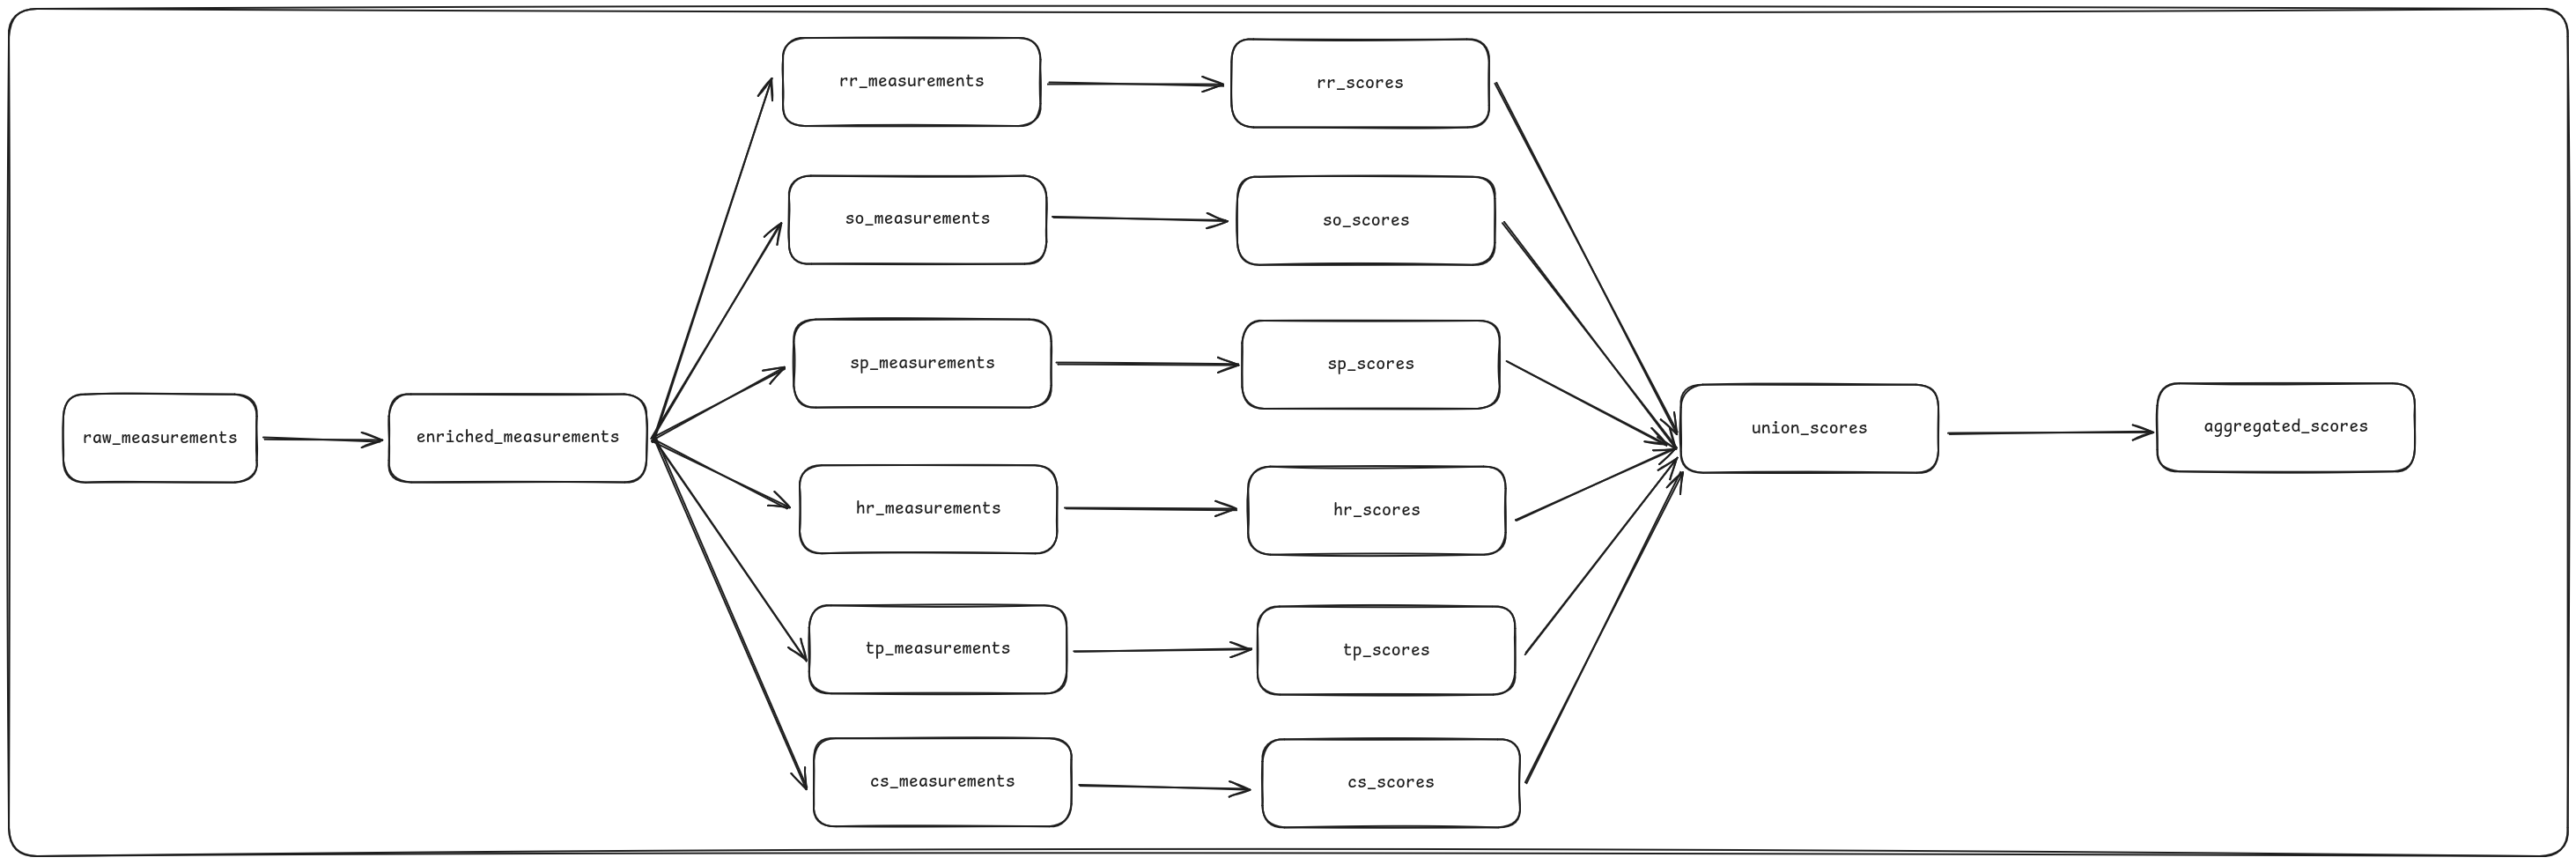
\includegraphics[width=\paperwidth]{desarrollo/pipeline.png}}
    \caption{Diagrama de flujo del pipeline de procesamiento}
    \label{fig:flowchart}
\end{figure}

\clearpage

\subsection{Despliegue de Componentes}

El despliegue de los componentes se realizó mediante el uso de \textbf{Docker Compose}, y se midió según las métricas expuestas por esta herramienta.
Por otro lado, para el calculo de costos, se asume un despliegue de alta disponibilidad en la nube de AWS basado en el siguiente diagrama:

\begin{figure}[h]
    \makebox[\textwidth]{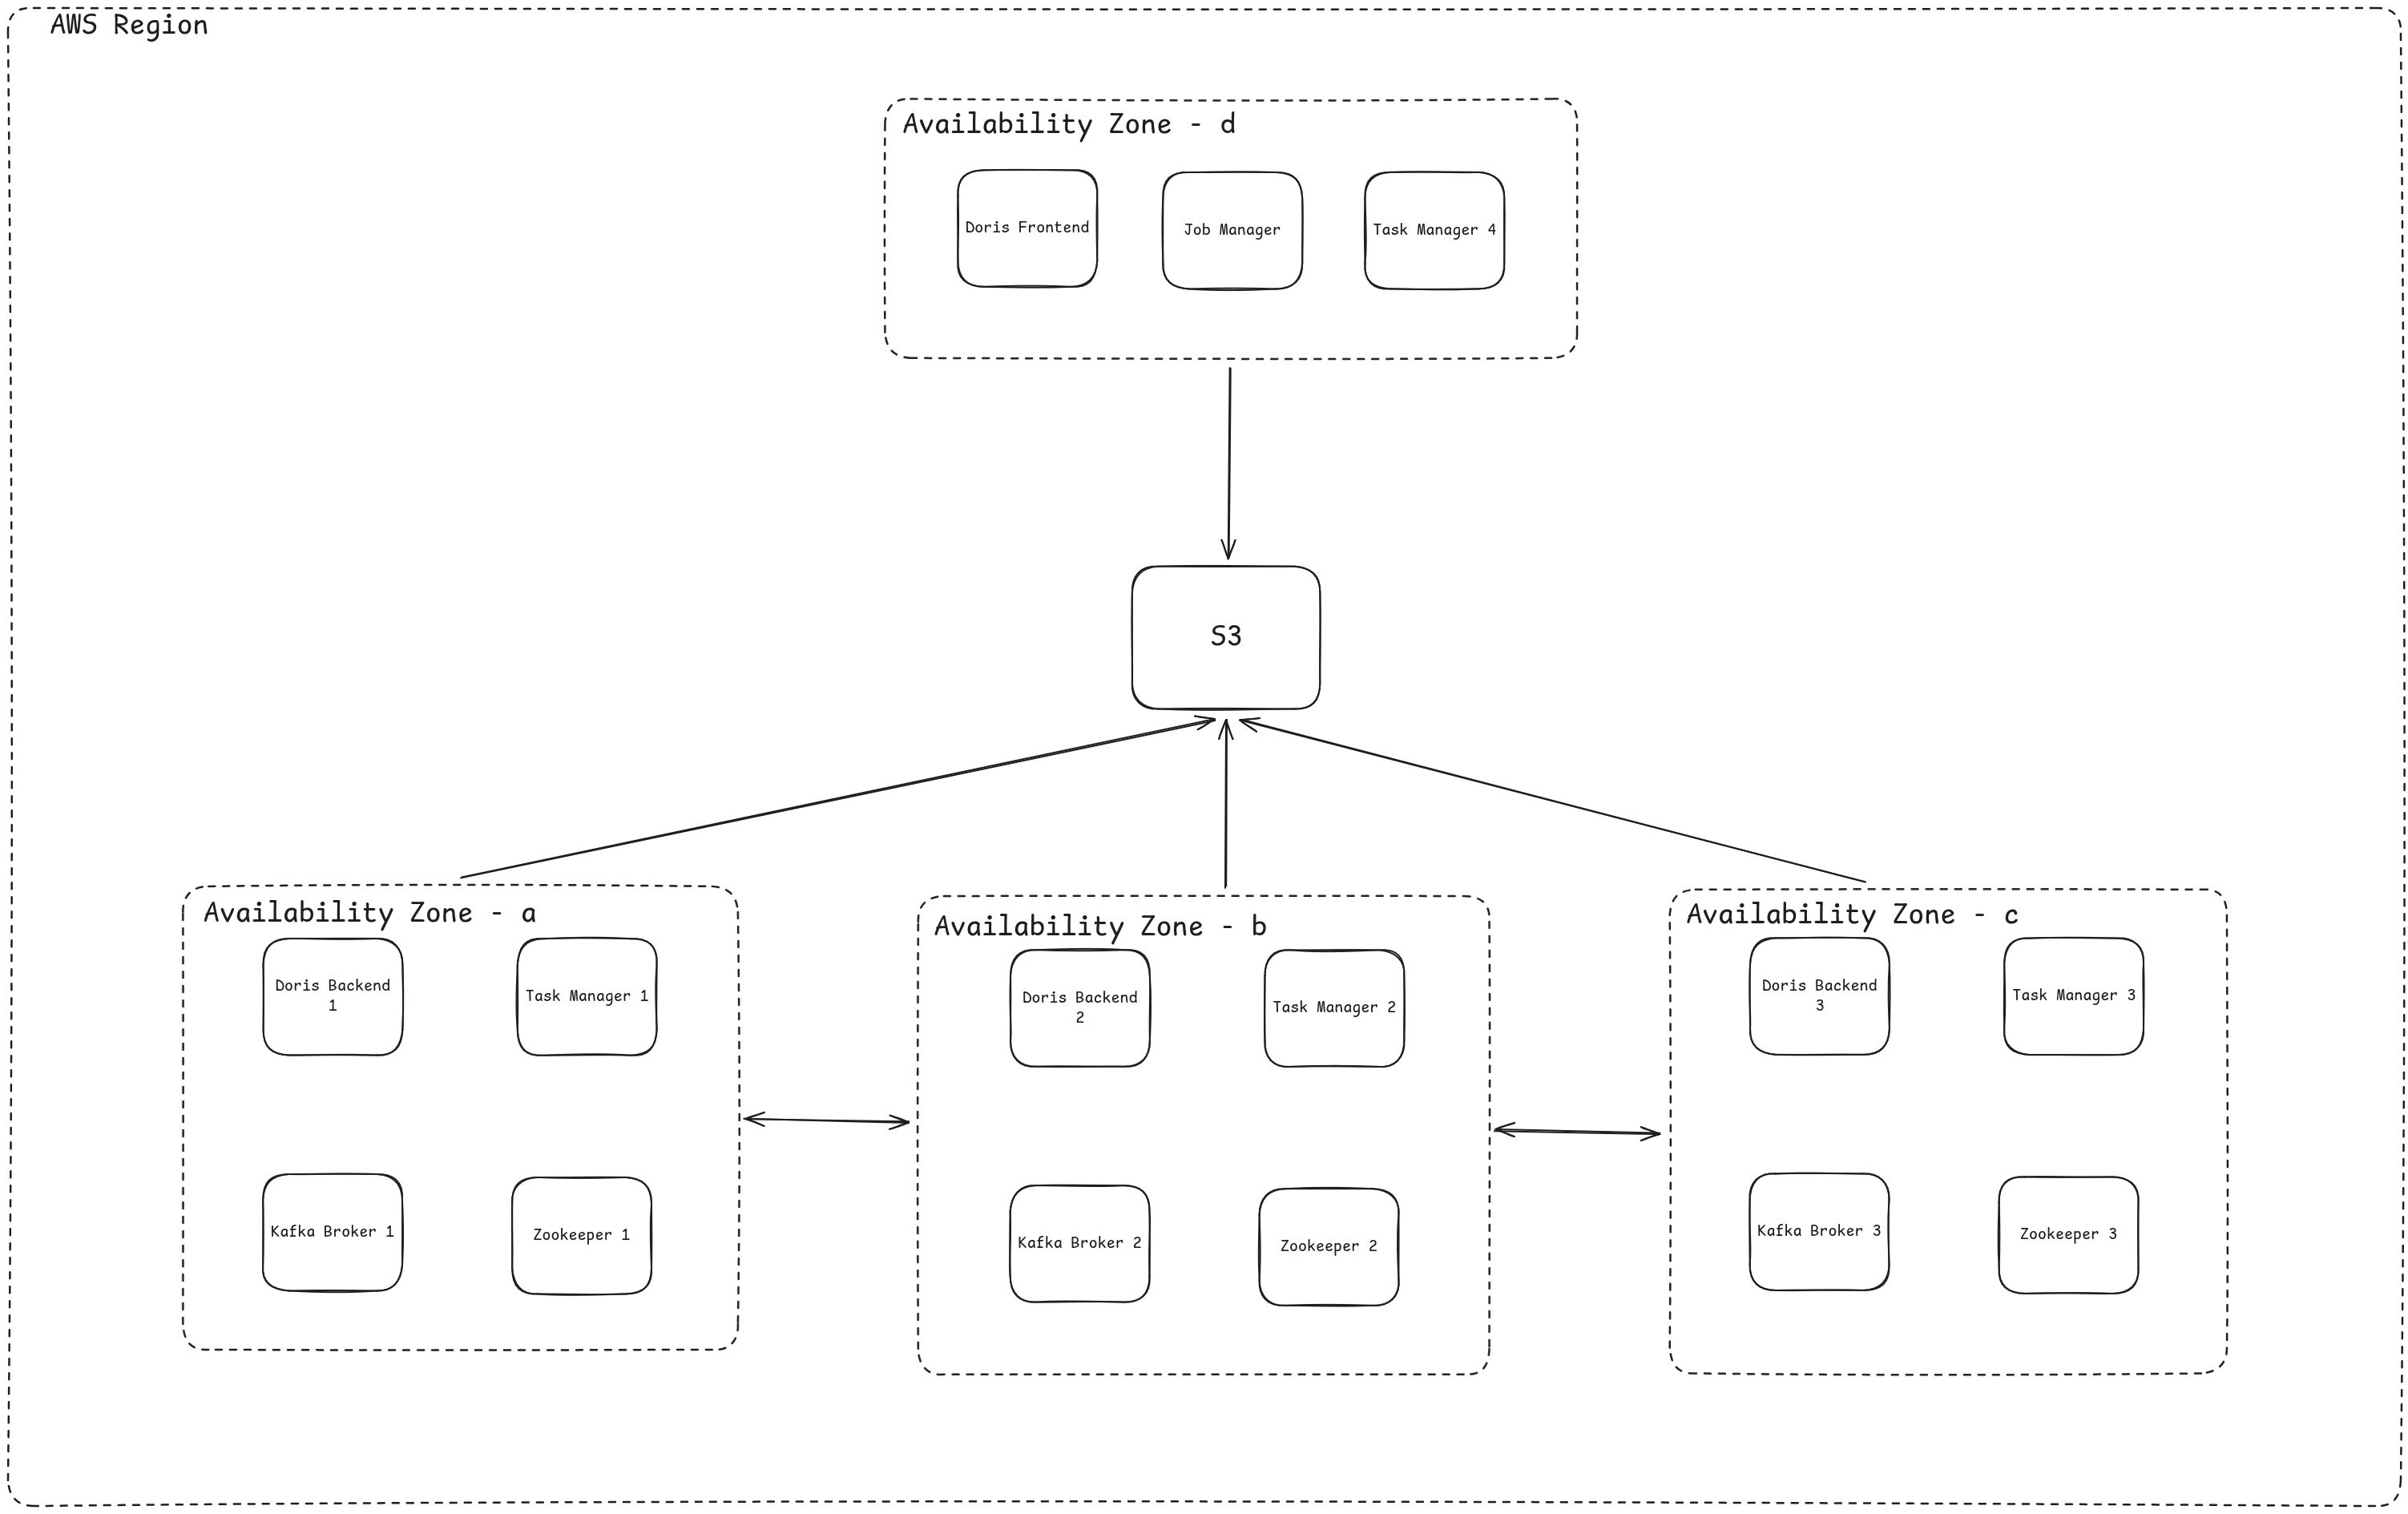
\includegraphics[width=\paperwidth]{desarrollo/deployment.png}}
    \caption{Diagrama de despliegue de componentes}
    \label{fig:infraestructura}
\end{figure}

\clearpage

La razón de este despliegue es la alta disponibilidad y la tolerancia a fallos, por lo que se despliega en una única región 
y se dividen los servicios en zonas de disponibilidad para asegurar que si una de ellas falla,
el sistema siga funcionando lo mejor posible.\newline

Tres de las zonas de disponibilidad (a, b y c) son idempotentes en cuanto a su funcionamiento, 
cada una cuenta con un nodo de Kafka, un nodo Zookeeper, un nodo de procesamiento de Flink y un nodo de backend de Doris.
La cuarta zona de disponibilidad (d) tiene el nodo de frontend de Doris y el nodo de gestión de Flink; así como también un nodo extra de procesamiento de Flink.
No se incluye MinIO en este despliegue porque se utiliza S3 nativo, que se define en una región y esta igualmente comunicado con todas las zonas de disponibilidad.\newline

A su vez, estarían idealmente desplegados mediante un orquestador de contenedores como Kubernetes, utilizando algún servicio como Elastic Kubernetes Serice (EKS).

\newpage

\subsection{Generación de Datos Sintéticos}

Se utilizaron datos sintéticos para realizar las pruebas de carga y estrés de ambas arquitecturas.
Para la generación de los datos sintéticos se utilizó un script en Python que permite definir perfiles de pacientes con diferentes características,
así como también el rango de tiempo para el que se genera la información.\newline

Se generaron datos sintéticos para 32 pacientes a lo largo de un año, con un total de 110.122.654 registros;
que implica un archivo CSV de aproximadamente 7GB.

El proceso de generación de datos es el siguiente:
\begin{itemize}
    \item Se genera un archivo CSV con los datos sintéticos ordenados por signo vital.
    \item Se separa este archivo CSV en un archivo por paciente y se ordena cada uno.
    \item Se vuelve a juntar la información de cada paciente de forma ordenada en un único archivo CSV.
    \item Se envía cada línea del CSV a los nodos Kafka de la cada una de las arquitecturas para su ingestión
\end{itemize}


Se debieron definir estos pasos debido al tamaño del archivo CSV, ya que al ser tan grande no se puede cargar en memoria.
Por otro lado, para simular demoras, se agregó una columna de delay al archivo inicial que luego fue tomada en cuenta al momento de ordenar las filas. 
El archivo CSV final resultante tiene el siguiente formato:
\begin{lstlisting}[language=CSV]
    device_id,measurement_type,timestamp,raw_value,battery,signal
    DEVICE_002_P0001,RESPIRATORY_RATE,-19.48,16.27,99.59,0.48
    DEVICE_002_P0001,TEMPERATURE,-3.46,36.43,99.67,0.72
    DEVICE_002_P0001,BLOOD_PRESSURE_SYSTOLIC,1.22,119.03,99.71,0.75
    DEVICE_002_P0001,HEART_RATE,3.0,70.31,99.8,0.71
    DEVICE_002_P0001,HEART_RATE,173.27,73.08,100.0,0.48
    DEVICE_002_P0001,RESPIRATORY_RATE,247.35,16.36,99.32,0.71
\end{lstlisting}

\newpage

El archivo de configuración usado tiene la siguiente forma: 

\begin{lstlisting}[language=JSON]
    {
        "time_range": "1_year",
        "patients": [
            {"patient_id": "P0001", "category": "HEALTHY"},
            ...
            {"patient_id": "P0005", "category": "ILL_STABLE"},
            ...
            {"patient_id": "P0009", "category": "HEALTHY_DETERIORATING"},
            ...
        ],
        "devices": [
            {
                "device_id": "MEDICAL_RR",
                "patient_ids": [
                    ...
                ],
                "vitals": {
                    "RESPIRATORY_RATE": {"measurement_rate": 60}
                },
                "battery": {"initial": 100, "drain_rate": 0.05},
                "signal_strength": {"base": 0.9, "variation": 0.1}
            },
            ...
            {
                "device_id": "CONSUMER_SMARTWATCH_002",
                "patient_ids": [
                    ...
                ],
                "vitals": {
                    "RESPIRATORY_RATE": {"measurement_rate": 240},
                    "BLOOD_PRESSURE_SYSTOLIC": {"measurement_rate": 300},
                    "HEART_RATE": {"measurement_rate": 180},
                    "TEMPERATURE": {"measurement_rate": 600}
                },
                "battery": {"initial": 100, "drain_rate": 0.02},
                "signal_strength": {"base": 0.6, "variation": 0.2}
            }
        ]
    }
\end{lstlisting}

\newpage

\subsection{Visualizaciones}

Se implementó un tablero de monitoreo utilizando Grafana, que permite visualizar la latencia, el throughtput y el uso de hardware en tiempo real.
Grafana se conecta con Prometheus que es el sistema de monitoreo utilizado para recolectar las métricas de los componentes de la arquitectura.

\begin{figure}[h]
    \centering
    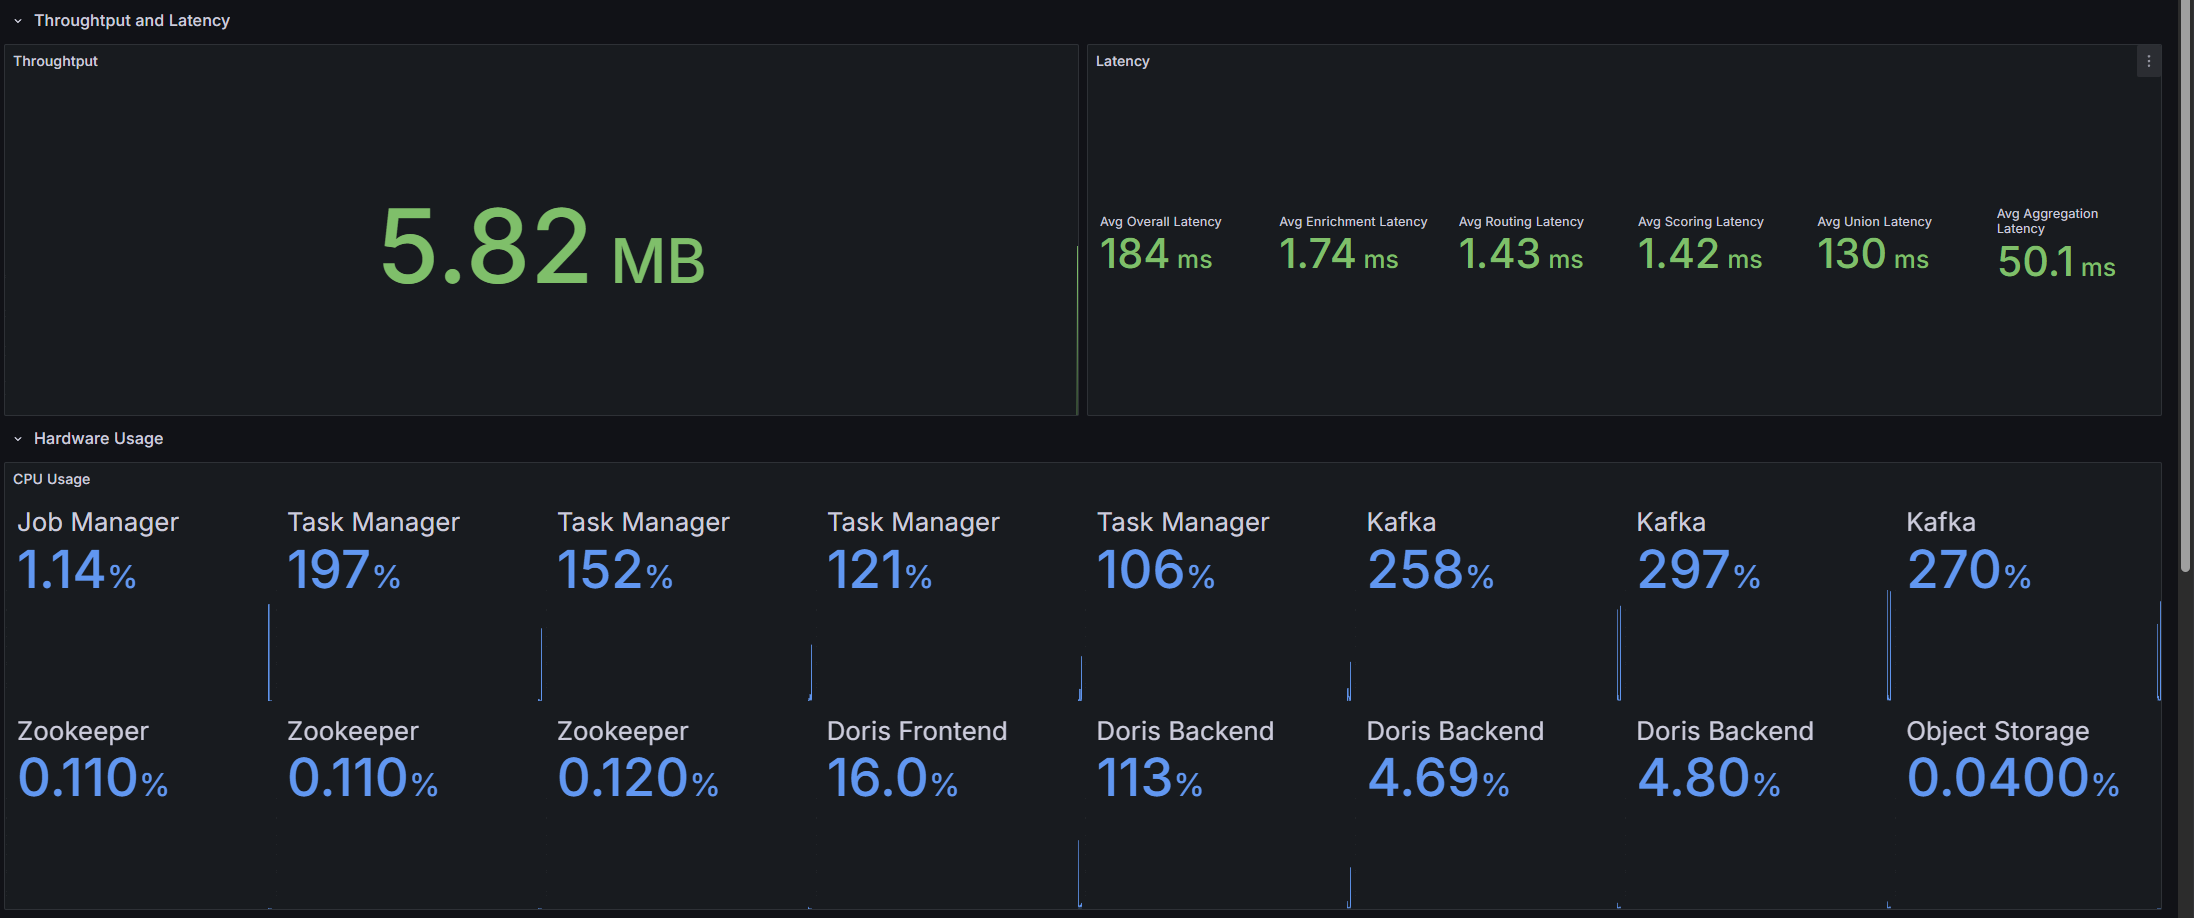
\includegraphics[width=1\textwidth]{desarrollo/monitoring1.png}
    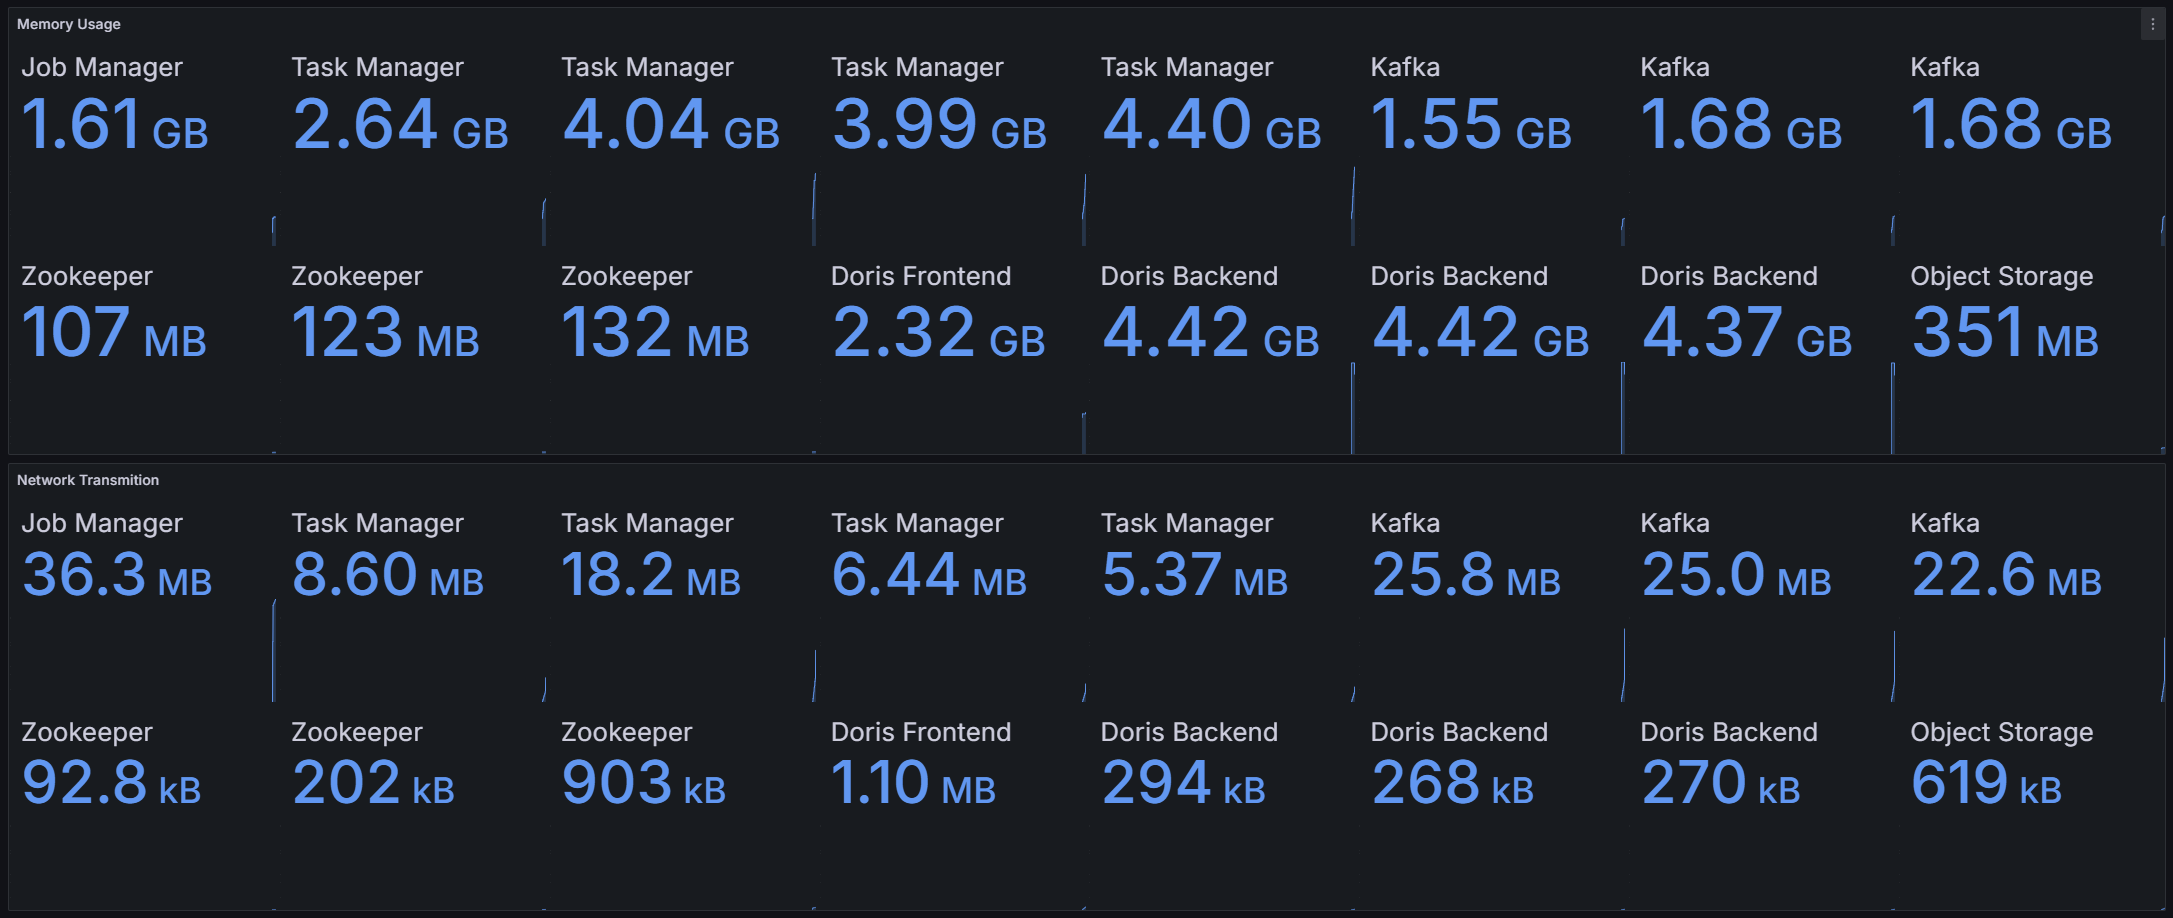
\includegraphics[width=1\textwidth]{desarrollo/monitoring2.png}
    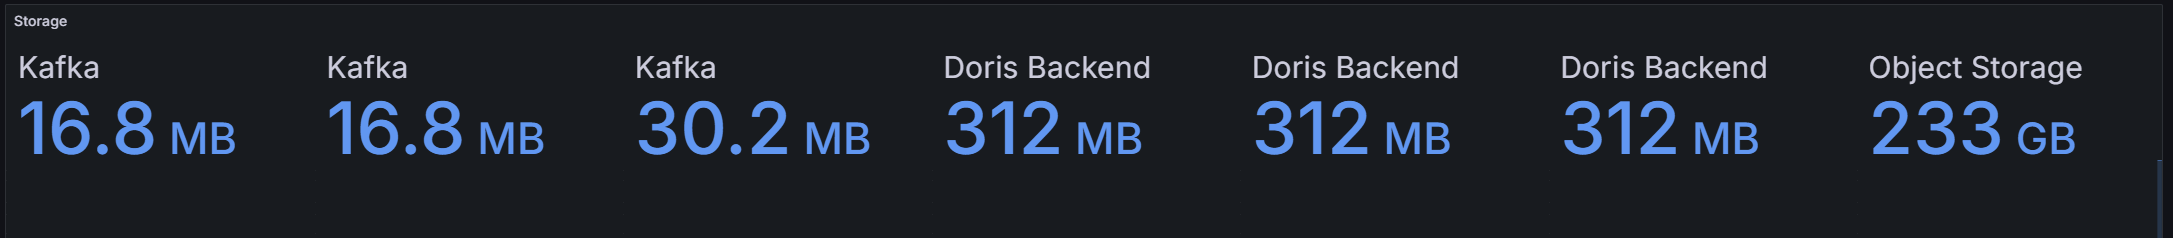
\includegraphics[width=1\textwidth]{desarrollo/monitoring3.png}
    \caption{Tablero de Monitoreo}
    \label{fig:monitoring}
\end{figure}
\clearpage

También se implementó en Grafana un tablero de datos por pacientes, que permite visualizar la evolución de los signos vitales de cada paciente a lo largo del tiempo.

\begin{figure}[h]
    \centering
    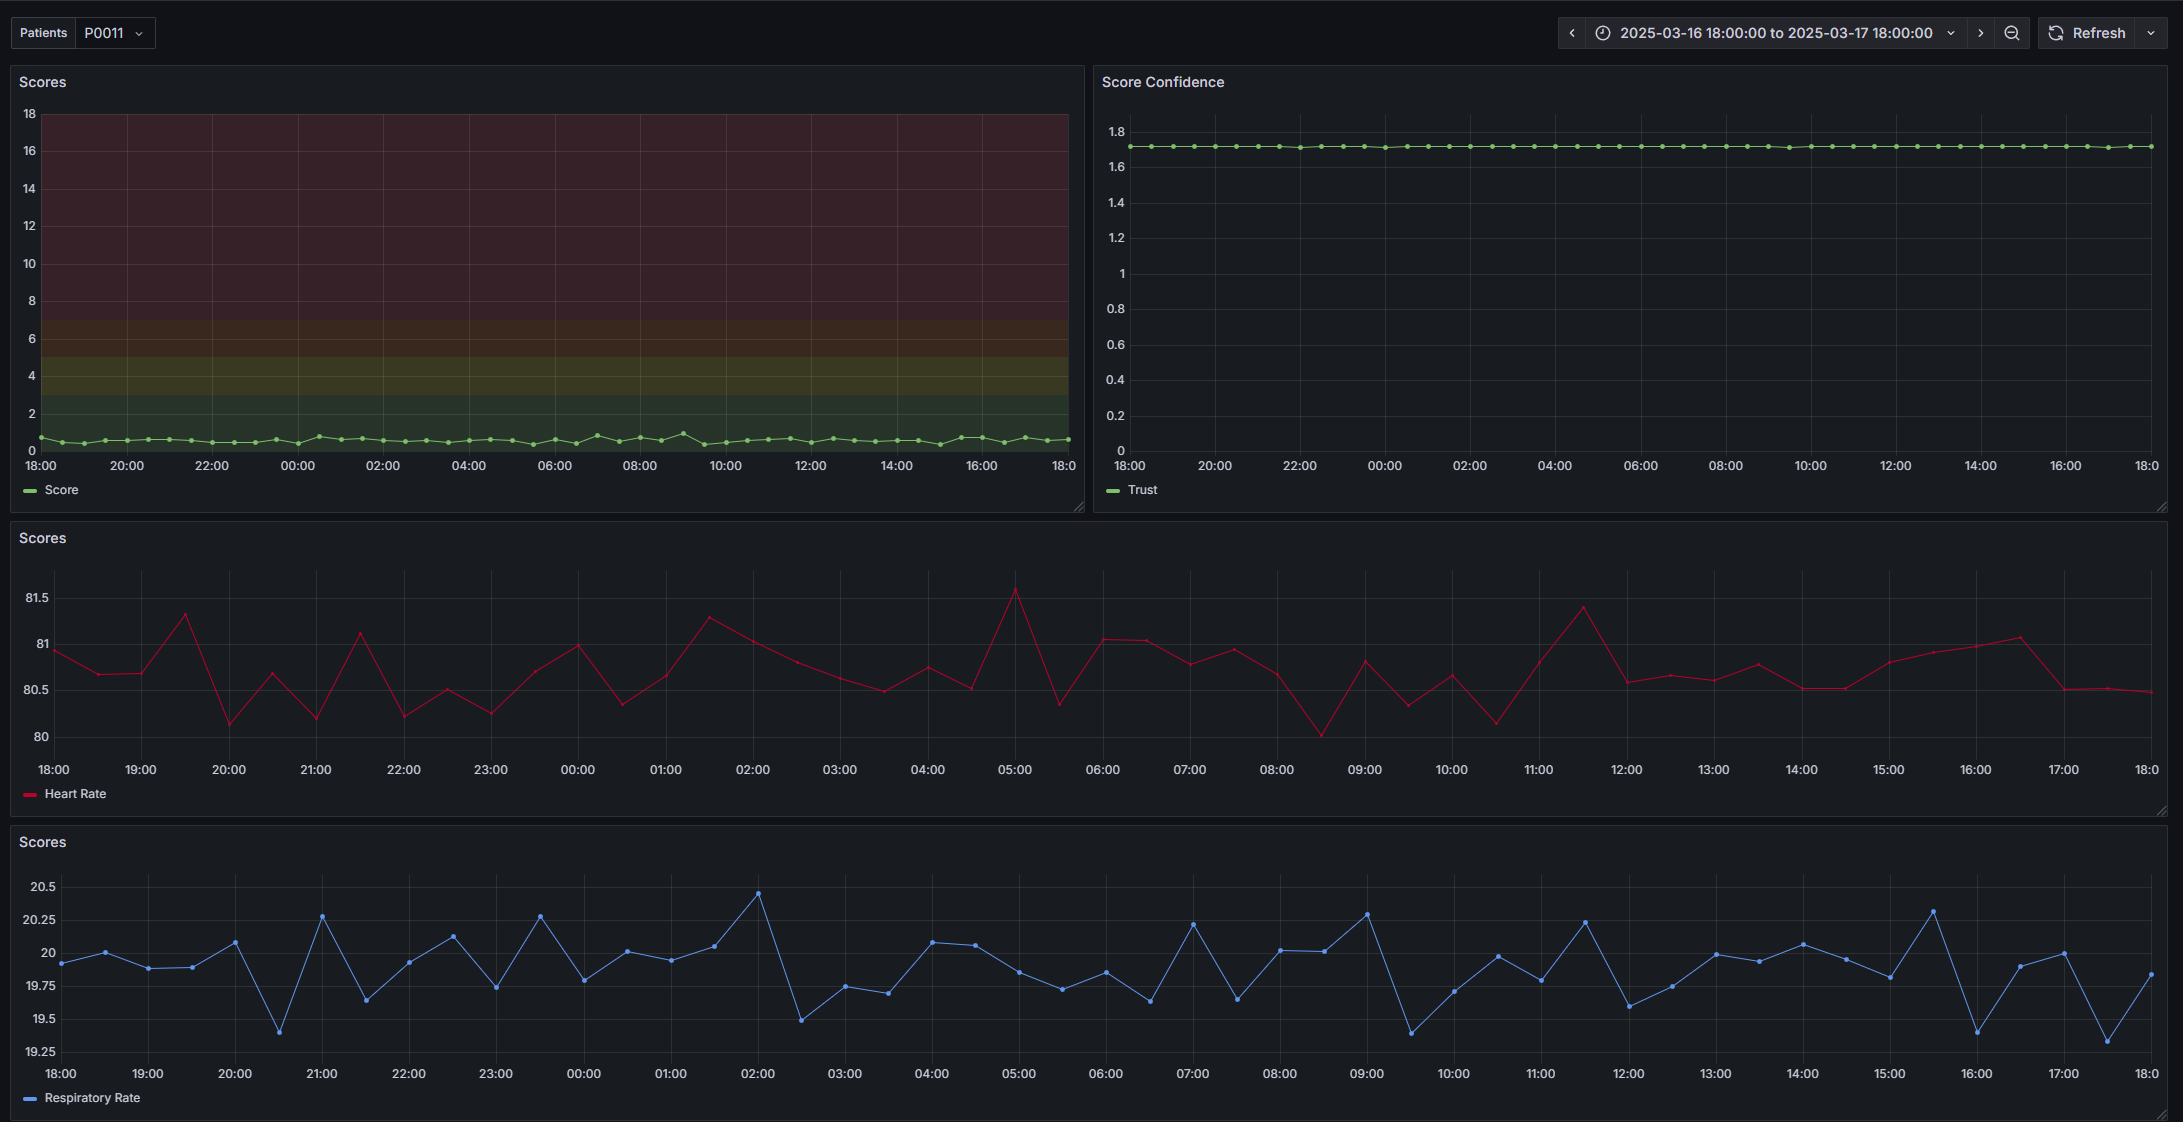
\includegraphics[width=1\textwidth]{desarrollo/visualization1.png}
    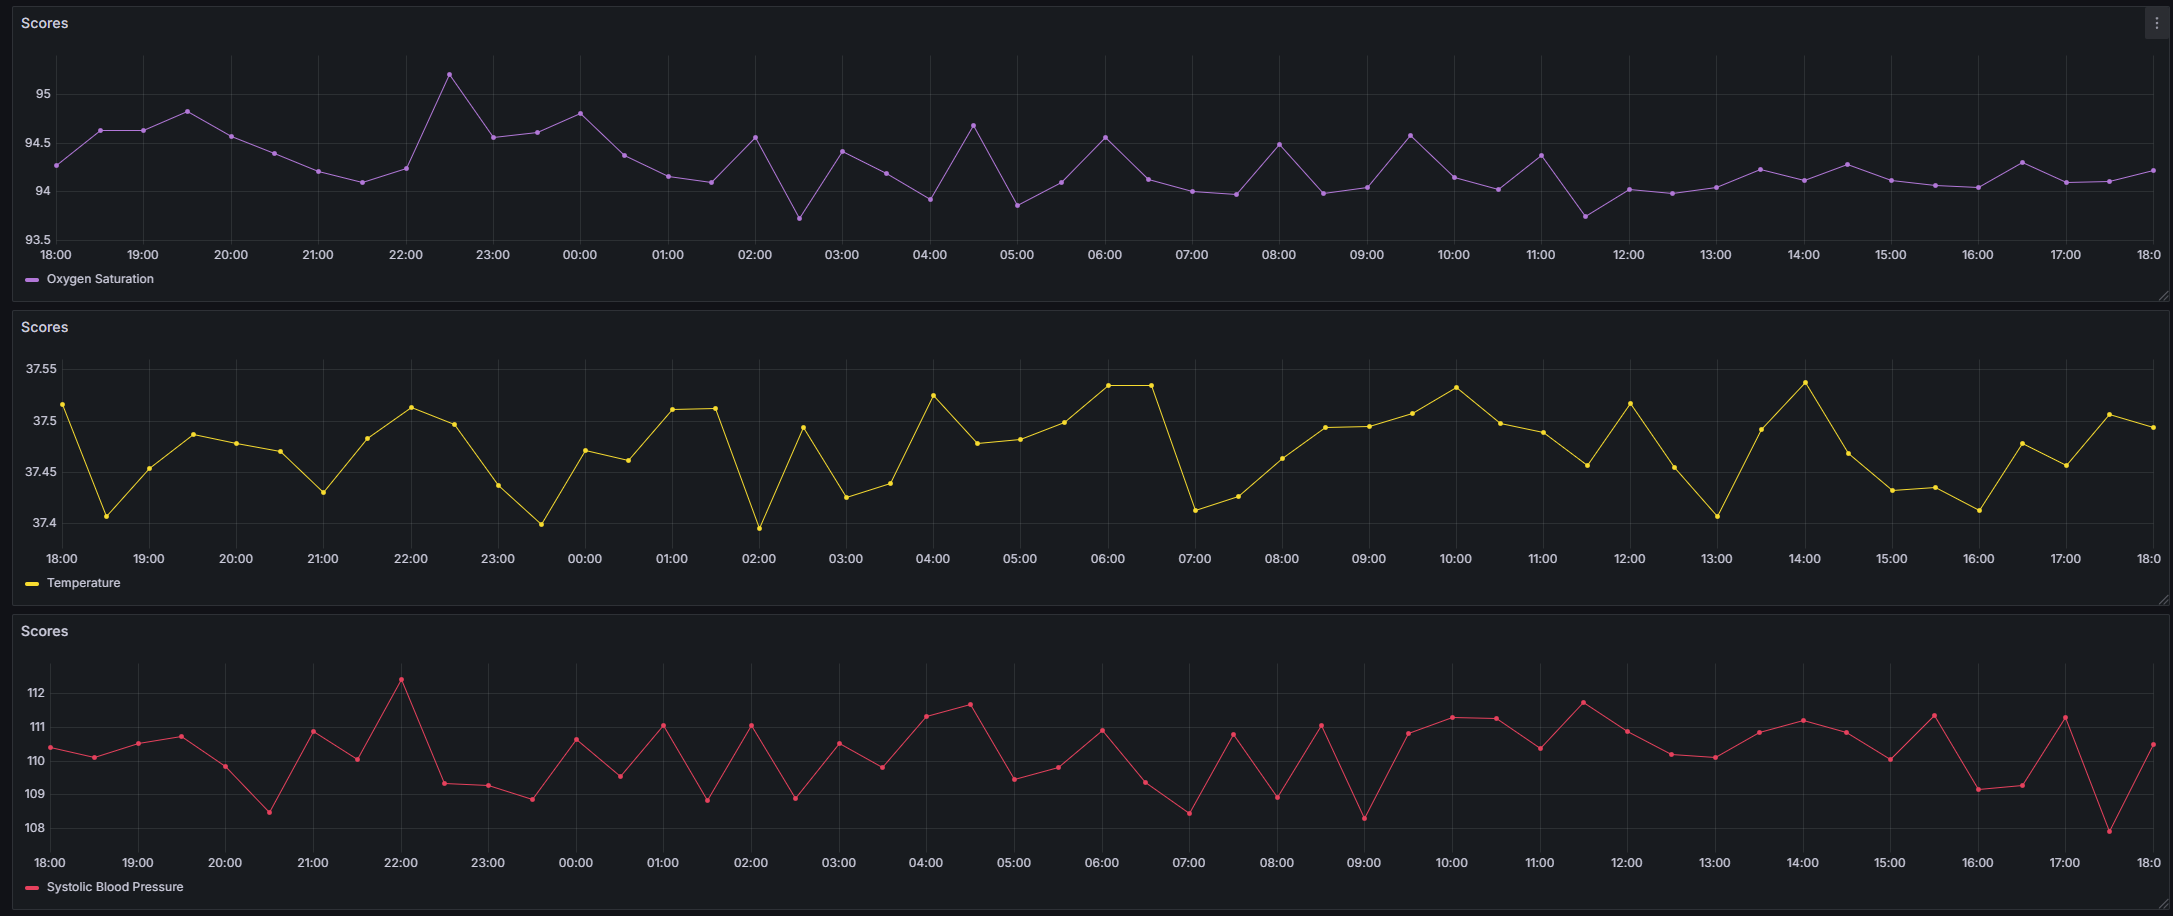
\includegraphics[width=1\textwidth]{desarrollo/visualization2.png}
    \caption{Tablero de Visualizaciones}
    \label{fig:visualization}
\end{figure}
\clearpage

\subsection{Limitaciones en la Implementación}

Se definieron algunas limitaciones en la implementación de la arquitectura Kappa y Delta, que se detallan a continuación:
\begin{itemize}
    \item No se implementará una solución de Governanza de datos
    \item No se implementará una solución de Calidad de Datos
    \item No se implementará una solución de Linaje de Datos
    \item No se implementará una solución de Gestión de Plataforma
    \item No se implementaron medidas de cifrado y anonimización de datos
\end{itemize}

Estas limitaciones se deben a que el objetivo de este trabajo es evaluar las arquitecturas Kappa y Delta,
e incluir esas soluciones haría que el trabajo se extienda mucho más allá de lo esperado.